\documentclass[11pt,a4paper]{amsart}
\usepackage[utf8]{inputenc}
\usepackage[T1]{fontenc}
\usepackage{lmodern}
\usepackage[english]{babel}
\usepackage{amsmath,amssymb,amsthm}
\usepackage[a4paper,textwidth=15.4cm,textheight=23.5cm,centering]{geometry}
\usepackage{booktabs}
\usepackage{enumitem}
\usepackage{microtype}
\usepackage{xcolor}
\usepackage{tikz}
\usetikzlibrary{shapes.misc}
\usepackage[colorlinks=true,linkcolor=blue!50!black,citecolor=blue!50!black,urlcolor=blue!50!black]{hyperref}
\usepackage{xurl}
\usepackage{array}
\setlength{\emergencystretch}{3em}
\raggedbottom
\setlist[enumerate]{leftmargin=2.2em}
\setlist[itemize]{leftmargin=1.6em}

\theoremstyle{plain}
\newtheorem{theorem}{Theorem}
\renewcommand{\thetheorem}{\Alph{theorem}}
\newtheorem{proposition}{Proposition}[section]
\newtheorem{lemma}[proposition]{Lemma}
\newtheorem{corollary}[proposition]{Corollary}
\newtheorem{question}[proposition]{Question}
\theoremstyle{definition}
\newtheorem{definition}[proposition]{Definition}
\newtheorem{remark}[proposition]{Remark}

\newcommand{\Q}{\mathbb{Q}}
\newcommand{\Z}{\mathbb{Z}}
\newcommand{\F}{\mathbb{F}}
\newcommand{\OO}{\mathcal{O}}
\newcommand{\Uc}{\mathcal{U}}
\newcommand{\Tc}{\mathcal{T}}
\newcommand{\q}{\mathfrak{q}}
\DeclareMathOperator{\Tr}{Tr}
\DeclareMathOperator{\Nm}{N}
\DeclareMathOperator{\Cl}{Cl}
\DeclareMathOperator{\Gal}{Gal}
\DeclareMathOperator{\Aut}{Aut}
\DeclareMathOperator{\Stab}{Stab}
\newcommand{\Lz}{L_{0}}
\newcommand{\LS}{L_{S}}
\newcommand{\st}[1]{\textup{\textsf{\small[#1]}}}
\newcommand{\DEM}{\st{proved}}
\newcommand{\GRH}{\st{under GRH}}
\newcommand{\ASS}{\st{computer-assisted}}
\newcommand{\CONS}{\st{observed}}
\newcommand{\HEUR}{\st{heuristic}}
\newcommand{\OUV}{\st{open}}
% genere par tableau_filtres.py ; audit de reference AUDIT_REJETS_20261017_044917.txt (sha256 7d3c6722f24f123b0500fb1741eb3c5b5b014d875e638e70682b6a87f01f66cf)
\newcommand{\nfiltres}{21}
\newcommand{\nrejets}{4}
\newcommand{\nsurv}{17}
\newcommand{\nfiltint}{10}
\newcommand{\nrejint}{3}
\newcommand{\nfiltext}{11}
\newcommand{\nrejext}{1}
\newcommand{\nsurvint}{7}
\newcommand{\nsurvext}{10}
\newcommand{\projmin}{4.3}
\newcommand{\projmax}{10.9}
\newcommand{\projminfr}{4{,}3}
\newcommand{\projmaxfr}{10{,}9}
\newcommand{\probint}{0.1}
\newcommand{\probext}{0.3}
\newcommand{\probintfr}{0{,}1}
\newcommand{\probextfr}{0{,}3}

% genere par statuts_recensement.py ; audit de reference AUDIT_REJETS_20261017_044917.txt (sha256 7d3c6722f24f123b0500fb1741eb3c5b5b014d875e638e70682b6a87f01f66cf)
\newcommand{\navant}{22}
\newcommand{\nouvertes}{18}
\newcommand{\coutavant}{830}
\newcommand{\coutheur}{660}
\newcommand{\couttous}{1\,700}

\newcommand{\lignesfiltresen}{%
$6$ & outer & $P_{1151}\sigma_{24}(P_{1151})$ & partial survivor & $4.3$ & $722$ &  \\
$12$ & inner & $P_{2531}\sigma_{24}(P_{2531})$ & rejected (side 2) & $0.2$ & $71$ & \rule[-1.6ex]{0pt}{4.4ex}$\frac{11913}{2531}+\frac{186878916}{5062^2}$ \\
$3$ & inner & $P_{3911}\sigma_{24}(P_{3911})$ & partial survivor & $6.0$ & $723$ &  \\
$11$ & outer & $P_{4831}\sigma_{24}(P_{4831})$ & partial survivor & $8.3$ & $722$ &  \\
$11$ & inner & $P_{5981}\sigma_{24}(P_{5981})$ & rejected (side 1) & $3.9$ & $315$ & \rule[-1.6ex]{0pt}{4.4ex}$\frac{28185}{5981}+\frac{1042775388}{11962^2}$ \\
$6$ & inner & $P_{6211}\sigma_{24}(P_{6211})$ & partial survivor & $7.1$ & $720$ &  \\
$9$ & inner & $P_{7591}\sigma_{24}(P_{7591})$ & partial survivor & $6.5$ & $722$ &  \\
$5$ & inner & $P_{8419}$ & partial survivor & $8.1$ & $721$ &  \\
$10$ & outer & $P_{8741}\sigma_{24}(P_{8741})$ & partial survivor & $7.6$ & $721$ &  \\
$14$ & inner & $P_{8971}\sigma_{24}(P_{8971})$ & partial survivor & $8.4$ & $720$ &  \\
$3$ & outer & $P_{9109}$ & partial survivor & $9.3$ & $721$ &  \\
$2$ & inner & $P_{9431}\sigma_{24}(P_{9431})$ & partial survivor & $7.8$ & $724$ &  \\
$1$ & outer & $P_{9661}\sigma_{24}(P_{9661})$ & partial survivor & $7.5$ & $720$ &  \\
$14$ & outer & $P_{14951}\sigma_{24}(P_{14951})$ & partial survivor & $10.1$ & $723$ &  \\
$4$ & outer & $P_{15319}$ & partial survivor & $10.9$ & $720$ &  \\
$10$ & inner & $P_{17389}$ & partial survivor & $8.7$ & $721$ &  \\
$1$ & inner & $P_{18401}\sigma_{24}(P_{18401})$ & rejected (side 1) & $0.2$ & $101$ & \rule[-1.6ex]{0pt}{4.4ex}$\frac{85506}{18401}+\frac{9959062824}{36802^2}$ \\
$7$ & outer & $P_{23599}$ & partial survivor & $9.4$ & $720$ &  \\
$9$ & outer & $P_{33581}\sigma_{24}(P_{33581})$ & partial survivor & $8.6$ & $720$ &  \\
$12$ & outer & $P_{39239}$ & rejected (side 2) & $1.8$ & $335$ & \rule[-1.6ex]{0pt}{4.4ex}$\frac{164472}{39239}+\frac{48090690576}{78478^2}$ \\
$0$ & outer & $P_{53269}$ & partial survivor & $9.0$ & $730$ &  \\
}


\title[Addendum: rank 88 over $\Q(\zeta_{115})$]{Addendum to ``Even unimodular ideal lattices of rank $88$ over $\Q(\zeta_{115})$'':\\ two further extremal lattices, an adversarial audit,\\ and the twins of the $\sigma_{24}$-layer}
\author{Ivan Gauvin}
\date{October 17, 2026}
\subjclass[2020]{Primary 11H06; Secondary 11H56, 11R18, 11R29}
\keywords{extremal lattices, even unimodular lattices, ideal lattices, cyclotomic fields, class group, certified enumeration}

\begin{document}

\begin{abstract}
This addendum to~\cite{Gau26} has three parts. (1) The ideal lattices $X_{4969}$ and $X_{4049}$, which~\cite{Gau26} listed as partial survivors of a filter, are extremal: their minimum $8$ is established by the computer-assisted method of~\cite{Gau26}, each of their four sides having been swept twice, with byte-identical receipts. Without assuming GRH, their ideal classes are conjugate neither to each other nor to those of $X_{139}$, $X_{599}$ and of Sakamoto's two lattices; by the isometry theorem of~\cite{Gau26}, six orbits of extremal lattices of rank $88$ are now known among the unimodular ideal lattices over $\Q(\zeta_{115})$. (2) The certified enumeration was attacked from seven sides: predicted hits, mutations, an independent recount, replications, a generic control group, a change of representative, and a review by a second assistant. (3) The $32$ orbits fixed by $\sigma_{24}$ are carried by the powers of a single prime ideal, $P_{139}^{\,k}$, and the orbit of an explicit ideal of this layer can be read without GRH; Sakamoto's lattice $\LS$ is isometric to the lattice of $P_{139}^{\,331}$. These orbits form sixteen \emph{twin pairs}, whose members differ by the class of Sakamoto's ideal. Twin certificates without GRH show that $X_{4049}$ and $X_{599}$ are twins, like $\Lz$ and $\LS$, whereas the twin of $X_{4969}$ contains a vector of norm $6$: extremality is not an invariant of twin pairs. Overnight filters on $\nfiltres$ of the $\navant$ undecided orbits of the layer rejected $\nrejets$ of them and left $\nsurv$ partial survivors, far more than a naive heuristic predicts.
\end{abstract}

\maketitle

\begin{center}
\fbox{\parbox{0.92\textwidth}{\small This addendum uses the notation and the five statuses of~\cite{Gau26}: \DEM, \GRH, \ASS, \CONS, \OUV, and \HEUR{} for a heuristic. A statement \ASS{} rests on the execution model of~\cite[\S5.4]{Gau26} (M1, M2, H1--H3). Numbered references such as~\cite[Prop.~2.5]{Gau26} are to the English version of the preprint.}}
\end{center}

\section{Summary}\label{sec:summary}
\enlargethispage{2\baselineskip}

\begin{theorem}[six extremal orbits]\label{thm:six}
The lattices $X_{139}$, $X_{599}$, $X_{4969}$ and $X_{4049}$ are even unimodular of rank $88$ and minimum $8$. They are pairwise non-isometric, and isometric neither to $\Lz$ nor to $\LS$. Together with Sakamoto's lattices, they form six pairwise distinct orbits of extremal lattices in the set $S$ of~\cite{Gau26}.

\st{minimum of $X_{4969}$, $X_{4049}$: computer-assisted (M1, M2, H1--H3), as for $X_{139}$, $X_{599}$ in~\cite[Thm.~6.11]{Gau26}; non-isometry: proved, without GRH, as in~\cite[Thm.~6.11]{Gau26}, by non-conjugacy of the classes and the isometry theorem; minimum of $\Lz$, $\LS$: by~\cite{Sak26}}
\end{theorem}

\begin{theorem}[extremality is not a twin invariant]\label{thm:twins}
In the $\sigma_{24}$-layer of $S$ (\S\ref{sec:layer}), the twin pairs $(\Lz,\LS)$ and $(X_{4049},X_{599})$ consist of two extremal lattices, whereas $X_{4969}$ is extremal and its twin, the lattice of the ideal $P_{691}\sigma_{24}(P_{691})$, contains a vector of norm $6$.

\st{twin relations and the vector of norm $6$: proved, without GRH; minima of $X_{4969}$, $X_{4049}$, $X_{599}$: computer-assisted; of $\Lz$, $\LS$: by~\cite{Sak26}}
\end{theorem}

\begin{theorem}[the dial without GRH]\label{thm:dial}
The $32$ orbits of $S$ fixed by $\sigma_{24}$ are those of the lattices $X_{P_{139}^{\,k}}$, $k\in\Z/993$, and they form $16$ twin pairs. The orbit of an explicit ideal of this layer can be determined without GRH; in particular, the $30$ non-central orbits are represented by ideals above the primes listed in Table~\ref{tab:census}, of norm at most $53\,269^2$.

\st{proved, without GRH, modulo~\cite[Prop.~2.2, 2.5]{Gau26}}
\end{theorem}

Theorem~\ref{thm:six} is proved in \S\ref{sec:new}, Theorems~\ref{thm:twins} and~\ref{thm:dial} in \S\ref{sec:layer} (Propositions~\ref{prop:cyclic}, \ref{prop:dial} and Corollaries~\ref{cor:twins}, \ref{cor:dial}). Question~(Q2) of~\cite{Gau26} is updated: at least six of the $508\,463$ orbits of $S$ consist of extremal lattices. Question~(Q3) is answered for two of the four partial survivors.

\begin{center}\small\renewcommand{\arraystretch}{1.2}
\begin{tabular}{>{\raggedright\arraybackslash}p{8.4cm}>{\raggedright\arraybackslash}p{6.2cm}}
\toprule
New statement & Status \\
\midrule
$X_{4969}$, $X_{4049}$: even unimodular; vector of norm $8$; explicit subgroup of order $460$ of the automorphism group (Prop.~\ref{prop:exact}) & proved (exact checks) \\
$X_{4969}$, $X_{4049}$: no non-zero vector of norm $\le6$ (Prop.~\ref{prop:sweeps}) & computer-assisted (H1--H3); each side executed twice, on two machines, identical receipts \\
Classes of $P_{4969}$, $P_{4049}$: order $993$, stabilizer $\langle\sigma_{24}\rangle$; non-conjugacy to $[P_{139}]$, $[P_{599}]$ and to each other (Prop.~\ref{prop:classes}) & proved, without GRH \\
Audit of the method (\S\ref{sec:audit}) & each item with its own status \\
The $\sigma_{24}$-layer is generated by $[P_{139}]$; $\LS\cong X_{P_{139}^{331}}$ (Prop.~\ref{prop:cyclic}) & proved, without GRH (modulo~\cite{Sak26} for $\LS$) \\
Twin pairing (Cor.~\ref{cor:twins}) & proved \\
Twin and same-orbit certificates (Prop.~\ref{prop:certs}) & proved, without GRH \\
$X_{P_{691}\sigma_{24}(P_{691})}$ contains a vector of norm $6$ (Prop.~\ref{prop:temoin}) & proved, without GRH \\
Labels and hours of the $30$ orbits of the layer (Prop.~\ref{prop:dial}, Cor.~\ref{cor:dial}) & proved, without GRH \\
Filters of the night on $\nfiltres$ orbits of the layer: $\nrejets$ rejections, $\nsurv$ partial survivors (\S\ref{subsec:census}) & rejections proved, without GRH; survivors observed \\
Enrichment of extremality in symmetric orbits (\S\ref{subsec:heur}) & heuristic \\
\bottomrule
\end{tabular}
\end{center}

\section{Two further extremal lattices}\label{sec:new}

\subsection{The ideals}
The primes $4969$ and $4049$ are congruent to $24$ modulo $115$. The prime ideals
\[
P_{4969}=(4969,\ \zeta^2+3763\zeta+2809),\qquad P_{4049}=(4049,\ \zeta^2+105\zeta+2084)
\]
have residue degree $2$, conjugates $\bar P_{4969}=(4969,\zeta^2+3189\zeta+1493)$ and $\bar P_{4049}=(4049,\zeta^2+1669\zeta+1327)$, and absolute norms $q=4969^2=24\,690\,961$ and $q=4049^2=16\,394\,401$. Their classes are fixed by $\sigma_{24}$, the Frobenius substitution of $p$. We set $X_p=(P_p,\beta_0/\nu)$ as in~\cite[\S6]{Gau26}. In~\cite[\S6.3]{Gau26}, $X_{4969}$ and $X_{4049}$ appear as partial survivors of a filter, after $3.8\%$ and $5.4\%$ of the tasks of one side.

\begin{proposition}\label{prop:exact}
For $p\in\{4969,4049\}$:
\begin{enumerate}[label=\textup{(\arabic*)}]
\item $X_p$ is a positive definite even unimodular lattice of rank $88$, and the input files of the certifying program are exactly linked to it, for both sides;
\item $X_p$ contains a vector of norm $8$;
\item the multiplication $g_1$ by $-\zeta$ and a semilinear map $g_2\colon u\mapsto\lambda\sigma_{24}(u)$, with $\lambda$ a unit of $\Z[\zeta]$, generate a subgroup of order $460$ of $\Aut(X_p)$, with $g_2^2=-1$ and $g_2^{-1}g_1g_2=g_1^{139}$.
\end{enumerate}
\DEM
\end{proposition}

\begin{proof}[Justification]
(1) The verifier of the geometric link of the repository of~\cite{Gau26}, the generic form of the one used for $X_{139}$ and $X_{599}$~\cite[Prop.~6.3, 6.4]{Gau26}, works in integers and rationals, without PARI/GP; it reports $37$ checks and no failure for each $p$. It checks that the basis generates exactly $P_p$ (index $p^2$, stability under $\zeta$, $P_p=(p,g(\zeta))$ with $g$ irreducible of degree $2$ modulo $p$, $P_p\ne\bar P_p$); that the Gram matrix, recomputed from $\alpha$, is integral, even, of determinant $1$ and positive definite; that $\nu$ generates $\Nm(P_p)$; the gluing identities of~\cite[Prop.~4.1]{Gau26}; for each side, the bijection between $P_p$ and the pairs $(u,y)$ and the identities that bind the four input files to the lattice; and that these four files are those whose hashes the first execution printed. The identity $\alpha\nu=\beta_0$, which this verifier took for granted, is checked by a separate verifier on the four lattices $X_{139}$, $X_{599}$, $X_{4969}$, $X_{4049}$ ($8$ checks, no failure; see \S\ref{subsec:review}).

(2) A short run of the certifying program on side~$1$, at the bounds $B_A=29/10$ and $S=16$ and stopped at the first hit, gives pairs $(u,y)$ of energies
\[
\frac{14\,083}{4969}+\frac{1\,300\,307\,796}{9938^2}=16\quad(p=4969),\qquad \frac{10\,194}{4049}+\frac{884\,139\,640}{8098^2}=16\quad(p=4049).
\]
The link verifier of~(1) checks that the reconstructed vectors have integer coordinates in the basis of the ideal and norm exactly $8$.

(3) The unit $\lambda$ solves $\alpha\lambda\bar\lambda=\sigma_{24}(\alpha)$; it was found by floating-point lattice reduction among explicit cyclotomic units, then checked exactly. The relations between $g_1$ and $g_2$ and the order $460$ were checked in exact arithmetic in PARI/GP, and again by two Python programs in integers and rationals (the scripts accompanying the data of $X_{139}$ and $X_{599}$, unchanged), which rebuild the Gram matrices and the generators from $P_p$, $\alpha$, $\lambda$ and the basis.
\end{proof}

\subsection{The certified sweeps}
The program \texttt{Rang88CertZ} of~\cite[\S5]{Gau26}, with the same compiled classes, was run on both sides of each ideal, with $B_A=1057/200$ and $S=12$, on rented machines with $32$ virtual cores (Scaleway, Ubuntu~24.04), from October~15 to~16, 2026. Each side was executed in a single launch, without resumption, then a second time on another machine (Table~\ref{tab:sweeps}). The parameters $(D_A,D_B,d)$ are $(4969,1,9938)$ and $(4049,1,8098)$.

\begin{table}[ht]
\caption{Certified sweeps of $X_{4969}$ and $X_{4049}$. Every execution: a single launch with a fresh checkpoint file, exit code $0$, empty error stream, complete coverage, no hit, no hit file. The canonical hash (SHA-256 of the receipts sorted by index) is the same for the two executions of each side, and so is the printed $|\Uc|$ with its histogram.}\label{tab:sweeps}
\centering\small\setlength{\tabcolsep}{2.8pt}
\begin{tabular}{lll rr l}
\toprule
side & first execution & replication & tasks & printed $|\Uc|$ & canonical hash \\
\midrule
$X_{4969}$, $1$ & AMS3, Java 21, $31\,240$ s & WAW1, Java 11, $31\,981$ s & $97\,270$ & $1\,544\,898\,536$ & \texttt{0226b9a5\dots} \\
$X_{4969}$, $2$ & AMS2, Java 21, $31\,312$ s & AMS3, Java 17, $29\,948$ s & $140\,082$ & $1\,544\,898\,536$ & \texttt{f6a1aecd\dots} \\
$X_{4049}$, $1$ & MIL1, Java 21, $47\,775$ s & AMS2, Java 21, $22\,286$ s & $77\,819$ & $1\,257\,946\,084$ & \texttt{6334d93e\dots} \\
$X_{4049}$, $2$ & MIL1, Java 21, $48\,258$ s & AMS2, Java 21, $25\,771$ s & $87\,731$ & $1\,257\,946\,084$ & \texttt{f95f16b8\dots} \\
\bottomrule
\end{tabular}

\smallskip
\begin{minipage}{0.95\textwidth}\footnotesize
Zones: Scaleway availability zones (Amsterdam 2 and 3, Milan 1, Warsaw 1). Java: OpenJDK 21.0.12.1, 17.0.20.1 and 11.0.32.1. Threads: $32$, except $15$ and $17$ for the first executions of $X_{4049}$. Durations: printed by the program.
\end{minipage}
\end{table}

For each of the eight executions, a read-only verifier, separate from the program and written for this addendum, rechecks: one launch with a fresh checkpoint file, complete selection, no resumption, the lines \texttt{TOTAL\_TOUCHES 0} and \texttt{COUVERTURE\_COMPLETE}, exit code $0$ and empty error stream; the hash of the task catalogue, against the log and the receipt header; the strict format of the receipts, the permutation of their indices, and \texttt{TOUCHES=0} on each of them; the agreement of their sums, histogram included, with the printed totals; the hash of the receipt file; the absence of hit files; the canonical hash, computed in two ways; and, for the replications, the byte-for-byte equality of each receipt with the corresponding receipt of the first execution. All checks pass ($27$ to $29$ per execution). The four replications reproduce all $402\,902$ receipts, without a single difference, under three versions of the Java virtual machine. The first executions also reproduce, byte for byte, the receipts of earlier partial runs on two other computers ($3\,716$ receipts for side~$1$ of $X_{4969}$, $8\,517$ and $4\,594$ for the two sides of $X_{4049}$). The enumeration trees are large: side~$1$ of $X_{4969}$ alone visits $1.07\cdot10^{12}$ nodes in rank $44$ for the short projections and $1.25\cdot10^{13}$ in the fibers.

\begin{proposition}\label{prop:sweeps}
$X_{4969}$ and $X_{4049}$ contain no non-zero vector of norm at most $6$. \ASS
\end{proposition}

\begin{proof}
For each of the four sides, Corollary~5.2 of~\cite{Gau26} applies to the fresh executions of Table~\ref{tab:sweeps}: exit code $0$, the line \texttt{COUVERTURE\_COMPLETE}, no hit file in the output directory (complete inventory taken after the end of the computation), and launch scripts that delete nothing. Hence $\Tc=\emptyset$ for each side, under H1--H3, and the criterion~\cite[Thm.~4.6]{Gau26}, with the geometric link of Proposition~\ref{prop:exact}, gives the claim. Hypothesis H4 plays no role.
\end{proof}

\subsection{Classes and non-isometry, without GRH}
Let $K=K_{22}=\Q(\theta)$, $\theta=\zeta+\zeta^{22}+\zeta^{24}+\zeta^{68}$, as in~\cite[\S6.4]{Gau26}, and $\q_p=P_p\cap K$; it has degree $1$, and $\Nm_{L/K}(P_p)=\q_p^2$.

\begin{proposition}\label{prop:classes}
For $p\in\{4969,4049\}$:
\begin{enumerate}[label=\textup{(\alph*)}]
\item $[P_p]$ has order $993$; its support is $\{3,331\}$, its stabilizer is $\langle\sigma_{24}\rangle$, and its orbit has size $44$;
\item $[P_p]$ is conjugate under $\Gal(L/\Q)$ neither to $[P_{139}]$, nor to $[P_{599}]$, nor to the class of the other ideal.
\end{enumerate}
\st{proved, without GRH, modulo~\cite[Prop.~2.2, 2.5]{Gau26}}
\end{proposition}

\begin{proof}
A certificate, verified by a Python program in exact arithmetic without PARI/GP, establishes the following, in the notation of~\cite[\S6.4]{Gau26}: an explicit $\Gamma_p\in K$ with $(\Gamma_p)=\q_p^{331}$, $\q_{4969}=(4969,\theta-4770)$, $\q_{4049}=(4049,\theta-512)$ (norm $p^{331}$, valuations at the $22$ primes above $p$); the rank $10$ of the discrete logarithms modulo $331$ of the units $\xi_2,\dots,\xi_{11}$ at the $88$ primes of degree $1$ above $\ell\in\{380\,651;\,1\,065\,821;\,1\,522\,601;\,2\,055\,511\}$, all $\equiv1\pmod{331\cdot115}$; the rank $11$ once the column of $\Gamma_p$ is added; and, for each of the $22$ elements $\tau$ of $\Gal(K/\Q)$, the rank $11$ for $\Gamma_p/\tau(\Gamma_{p'})$, with $p'=139$, and also $p'=4969$ when $p=4049$. The verifier reports $39$ checks for $P_{4969}$ and $49$ for $P_{4049}$, no failure; they include an autonomous check that the basis of the input files generates $P_p$ (index $p^2$).

(a) The rank $11$ and Steps~1--3 of~\cite[\S6.4]{Gau26} show that $P_p^m$ is not principal for $m$ prime to $331$: the $331$-component is non-zero. The prime $p$ is $\equiv1\pmod{23}$, hence splits in $F=\Q(\sqrt{-23})$, and $4p$ is not of the form $a^2+23b^2$ ($4\cdot4969=19\,876$, $4\cdot4049=16\,196$): the prime $\mathfrak p$ of $F$ above $p$ is not principal, nor is $\Nm_{L/F}(P_p)=\mathfrak p^2$, and the $3$-component is non-zero, by the argument of~\cite[Rem.~6.8(a)]{Gau26}. The $45\,013$-component vanishes because $\sigma_{24}$ fixes $P_p$ and does not lie in the kernel of $\chi_{45\,013}$. As in~\cite[Rem.~6.8(a)]{Gau26}, the order is $993$, the stabilizer is $\ker\chi_3\cap\ker\chi_{331}=\{1,24\}$ and the orbit has size $44$.

(b) If $[P_p]=\sigma[P_{p'}]$ for some $\sigma\in\Gal(L/\Q)$, then, taking norms to $K$, $\q_p^2\,\tau(\q_{p'})^{-2}$ would be principal, with $\tau=\sigma|_K$, and $\Gamma_p^2/\tau(\Gamma_{p'})^2$ would lie in $E\cdot K^{\times331}$; Step~1 and the rank $11$ forbid this, exactly as in Step~2 of~\cite[\S6.4]{Gau26}. Finally $[P_{599}]$ has zero $3$-component~\cite[Prop.~6.7]{Gau26}, whereas $[P_p]$ has not.
\end{proof}

\begin{proof}[Proof of Theorem~\ref{thm:six}]
Evenness, unimodularity and the vector of norm $8$: Proposition~\ref{prop:exact} and~\cite[Prop.~6.3, 6.4]{Gau26}. Minimum $\ge8$: Proposition~\ref{prop:sweeps} and~\cite[Thm.~6.11]{Gau26}; hence minimum $8$. Non-isometry: the classes $[P_{139}]$, $[P_{599}]$, $[P_{4969}]$, $[P_{4049}]$ are pairwise non-conjugate (Proposition~\ref{prop:classes} and~\cite[Rem.~6.10]{Gau26}), and none of their cubes is trivial, whereas those of the classes of $\Lz$ and $\LS$ are~\cite[Prop.~2.7]{Gau26}. The isometry theorem~\cite[Thm.~3.3]{Gau26} applies to lattices of minimum at least $8$; all six have minimum $8$, so it turns non-conjugacy into non-isometry. As in~\cite[Prop.~6.9(a)]{Gau26}, the non-isometry to $\Lz$ and $\LS$ does not even need the computer-assisted minimum: a lattice of minimum at most $6$ is not isometric to a lattice of minimum $8$.
\end{proof}

\begin{remark}
By~\cite[Rem.~2.6]{Gau26} and Proposition~\ref{prop:classes}, the subgroup of Proposition~\ref{prop:exact}(3) is the full normalizer of the group of multiplications by roots of unity: $|\Aut(X_{4969})|\ge460$ and $|\Aut(X_{4049})|\ge460$. Gram matrices in LLL-reduced bases, the two generators and the vectors of norm $8$ have been prepared in the format of the Catalogue of Lattices~\cite{NS}, as for $X_{139}$ and $X_{599}$.
\end{remark}

\section{Attacks on the method}\label{sec:audit}

A computer-assisted statement is worth the attacks it has survived. On October~16, 2026, the certifying pipeline was attacked deliberately, each attack aimed at one way in which a certified enumeration can fail. The second assistant, Astra, designed part of the plan, reviewed the records, and was asked to look for flaws. Table~\ref{tab:audit} gives the outcome; each line is detailed below.

\begin{table}[ht]
\caption{Seven attacks on the certified enumeration (October 16--17, 2026).}\label{tab:audit}
\centering\small\renewcommand{\arraystretch}{1.15}
\begin{tabular}{>{\raggedright\arraybackslash}p{2.9cm}>{\raggedright\arraybackslash}p{6.1cm}>{\raggedright\arraybackslash}p{5.1cm}}
\toprule
failure mode & attack & outcome \\
\midrule
blindness to existing vectors & predict the hits from known witnesses of norm $6$ and their $115$ rotations, by a PARI/GP script that reads no output of the program; replay only the tasks concerned & $334$ of $334$ predicted hits found, on $7$ rejected lattices and $14$ sides, plus $22$ exact hits of other orbits; one hit $3\cdot10^{-5}$ below the threshold \\
rounding and pruning & $8$ single mutations of the source (leaf test, budgets, outward roundings, fixed point, zero vector, signs) & $3$ killed by the tests, $1$ without effect; $4$ survive every finite test: only the non-omission proof covers them \\
counting & recount $|\Uc|$ of $X_{139}$, side $1$, with \texttt{qfminim} of PARI/GP & identical at $6$ thresholds, including $42\,957\,972$ at $1057/200$ \\
machine, hardware & replicate each side of $X_{4969}$, $X_{4049}$ on another machine (another Java version for $X_{4969}$) & $402\,902$ receipts, $0$ differences \\
dependence on coordinates & sweep a different ideal of the orbit of $X_{139}$, proved conjugate without GRH & $X_{P_{461}\sigma_{24}(P_{461})}\cong X_{139}$: no hit on either side \\
generic behaviour & $16$ degree-$1$ ideals, filter with stop at the first hit & $14$ rejected in less than $5$ minutes each ($3$ already rejected by PARI/GP), $2$ partial survivors \\
blind spots of the author & adversarial review by a second assistant & no serious flaw of the preprint; two gaps in the verifiers and a defect in a new verifier, all corrected \\
\bottomrule
\end{tabular}
\end{table}

\subsection{Sensitivity: predicted hits}
For seven rejected lattices of~\cite[Table~2]{Gau26} ($P_{691}$, $P_{1151}$, $P_{1381}$ of degree $1$; $P_{829}$, $P_{1289}$, $P_{1471}$, $P_{1979}$ of degree $2$), a PARI/GP script computed, from the published witness $z$ of norm $6$ and its rotations $\zeta^kz$, the exact pairs $(u,y)$ of both sides that the criterion must catch, and checked on them the identities of~\cite[\S4]{Gau26} (zero mean, the $23$ relations with five terms, Parseval, $\max|f|\ge N\sqrt{5/352}$). It reads no output of the Java program. Each predicted $u$ lies in exactly one task of the catalogue, which is thus checked to be a partition on these vectors. The tasks containing the predicted $u$ were then replayed without stopping at the first hit: the $334$ predicted hits were all found, with the same $u$, $y$ and energies, together with $22$ further hits, all of exact norm $6$, from other orbits. On side~$1$ of $P_{1151}$, a predicted hit of short energy $6083/1151\approx5.28497$ lies $3\cdot10^{-5}$ below the threshold $1057/200$ (and above the Parseval value $6-\sqrt{45/88}\approx5.28490$); it is found. For the four lattices of degree~$2$, the starting witness had itself been found by a Java program (by \texttt{Rang88CertZ} for three of them); the prediction of the other $114$ rotations and of side~$2$, and the exact check of the extra hits, do not depend on it. In a boundary variant, where $B_A$ is set exactly to the energy of the highest predicted hit of a side, the reference program finds all hits, including the one on the boundary. \CONS

\subsection{Mutations}
Eight copies of the source were made, each with a single substitution, and run against three tests: the test harness of the program ($910$ checks), the validation of~\cite[\S5.2]{Gau26} on $P_{461}$ at threshold $7/2$ ($697$ short projections, $2$ hits), and the replay of $12$ tasks of $X_{4969}$ against reference receipts; then against the boundary variant above. Three mutants are killed: the leaf test without equality, a fiber budget lowered by one step, and a change of the sign convention. A fourth, which no longer excludes the zero vector at the last level, has no effect: the zero vector is excluded a second time at the leaf. The four others prune as soon as the remaining budget is zero, remove the outward rounding of the remaining budget or of the radius, or shrink an integer range by one unit of $2^{-40}$ in fixed point. They pass every test, even at the exact boundary. No finite test of this kind can see them; the correctness of the code they modify rests on the non-omission proof alone (lemmas Z3--Z5, outward rounding L3, model M1). For the first of them, the author's argument, a lower bound on the budget, did not hold in general; Astra replaced it by an invariant of the program, namely that the accumulated partial energy never exceeds the current bound (\texttt{PL}~$\le$~\texttt{borneU}) on any reachable call, so that the value at which the two versions differ is never reached. This experiment does not weaken the proof; it shows where only the proof protects. \CONS

\subsection{An independent recount}
The number $|\Uc|$ of short projections of side~$1$ of $X_{139}$ was recounted with \texttt{qfminim} of PARI/GP, another program by other authors, on the same integer Gram matrix. For short energies below $3$, $7/2$, $4$, $9/2$ and $5$, and at most $1057/200$, it gives $162$, $4\,878$, $92\,734$, $1\,260\,158$, $12\,651\,642$ and $42\,957\,972$, exactly the values printed by \texttt{Rang88CertZ}; the last count took $11\,260$~s. \texttt{qfminim} is not certifying, but it is an enumerator independent of the Java code. \CONS

\subsection{Replications}
Each side of $X_{4969}$ and $X_{4049}$ was executed twice, on different rented machines, under OpenJDK~21, 17 and 11 (Table~\ref{tab:sweeps}). The $402\,902$ receipts of the four replications are byte-identical to those of the first executions. Together with the replications of~\cite{Gau26}, every side of the four extremal lattices of Theorem~\ref{thm:six} has now been executed twice with identical receipts. These replications support H2 and H3 without proving them; they share the program, and they are not an independent implementation.

\subsection{Change of representative}
The ideal $I=P_{461}\sigma_{24}(P_{461})$, with $P_{461}=(461,\zeta-5)$, has norm $461^2$ and the same orbit as $P_{139}$ (Proposition~\ref{prop:certs}(c) below, without GRH): $X_I$ is isometric to $X_{139}$, but its ideal, basis, Gram matrix, input files and task catalogue are all different. Its two sides were swept completely on October~16 ($73\,244$ and $73\,359$ tasks, $9\,559$~s and $8\,750$~s, $16$ threads each, exit code $0$, complete coverage, no hit; $27$ checks of the verifier per side). The printed $|\Uc|$ is $143\,529\,602$ on each side, against $42\,957\,972$ for $X_{139}$: a different tree, the same verdict. This is a second, computer-assisted proof of the minimum of $X_{139}$ (one execution per side). Conversely, the ideals $P_{1381}\sigma_{24}(P_{1381})$, $P_{3221}\sigma_{24}(P_{3221})$ and $P_{5521}\sigma_{24}(P_{5521})$, in the orbits of the rejected $P_{1289}$, $P_{1979}$ and $P_{829}$ (Proposition~\ref{prop:certs}(d)), gave hits within less than nine minutes; the four hit vectors (two for the second ideal) were checked to have exact norm $6$.

\subsection{A generic control group}
The sixteen smallest primes $p\equiv1\pmod{115}$ after $461$ give ideals $(p,\zeta-r)$ of degree $1$, a priori in generic orbits of size $88$. A filter on side~$1$ (author's computer, Java~11, $8$ threads), stopped at the first hit and capped at $300$~s, rejected $14$ of them, after $33$ to $941$ tasks: the three already rejected in~\cite{Gau26} by its PARI/GP filter, and eleven new ones. Two, $P_{2531}$ and $P_{11731}$, are partial survivors; for $P_{2531}$, the PARI/GP filter of~\cite{Gau26} had also stopped without a decision. Some rejections required about a thousand tasks: a short filter must cover at least a few thousand of them. \CONS

\subsection{Review}\label{subsec:review}
Astra (OpenAI) had the records attacked by separate agents and reread their reports itself, under fixed hashes: the non-omission proof and its link to the code (zero budgets, conversions, underflow, boundaries, overflow, cache, partition of the tasks, hits; $296$ local exact comparisons, without running the Java program); the isometry theorem; the geometric links and the class certificates of $X_{4969}$ and $X_{4049}$; and the records of their four first executions (exit codes, error streams, archives and inventories of the output directories, in which there is no hit file). It made its own exact checks of $\alpha\nu=\beta_0$ on the four lattices and of the fiber identities on the eight sides. Its conclusion: no serious flaw of the preprint was established. It reported two minor points of presentation in the non-omission proof; that the link verifier asserted $\alpha\nu=\beta_0$ without testing it (the identity holds, and is now tested); that one check of the class certificates identified the basis with the prime ideal only through the link verifier (the certificate now contains its own index test); and a real defect in a verifier written during the audit, a Newton identity that counted one term twice, which was corrected and reread. Astra's review does not certify the minimum of $X_{4969}$ and $X_{4049}$, and does not claim to. It leaves open what~\cite[\S5.4]{Gau26} leaves open: no independent implementation of the enumeration, and H3.

\section{The twins of the \texorpdfstring{$\sigma_{24}$}{sigma24}-layer}\label{sec:layer}

\subsection{All $\sigma_{24}$-stable lattices are powers of one ideal}
Let $\Cl(L)^{\sigma_{24}}$ be the subgroup of the classes fixed by $\sigma_{24}$. By~\cite[Prop.~2.5]{Gau26}, $\sigma_{24}$ lies in the kernels of $\chi_3$ and $\chi_{331}$, not in that of $\chi_{45\,013}$; hence $\Cl(L)^{\sigma_{24}}=\Cl_3\times\Cl_{331}$, cyclic of order $993$. It contains the classes of the prime ideals of degree~$2$ above the primes $p\equiv24\pmod{115}$, those of the ideals $P\sigma_{24}(P)$, and those of Sakamoto's two lattices. We identify $\Z/993$ with $\Z/3\times\Z/331$.

\begin{proposition}[cyclic layer]\label{prop:cyclic}
\begin{enumerate}[label=\textup{(\alph*)}]
\item The class $[P_{139}]$ generates $\Cl(L)^{\sigma_{24}}$: every $\sigma_{24}$-stable element of $S$ is $X_{P_{139}^k}$ for a unique $k\in\Z/993$.
\item For $a$ prime to $115$, $\sigma_a[P_{139}]^k=[P_{139}]^{\varepsilon(a)k}$, where $\varepsilon(a)=(\chi_3(a),\chi_{331}(a))$ runs over the whole group $H=\{\pm1\}\times\mu_{22}$ of $(\Z/3)^\times\times(\Z/331)^\times$. The $32$ orbits of $S$ fixed by $\sigma_{24}$ are the orbits of $H$ on $\Z/993$:
\[
\{0\},\qquad\{331,662\},\qquad 15\ \text{orbits with}\ 3\mid k,\ 331\nmid k,\qquad 15\ \text{orbits with}\ 3\nmid k,\ 331\nmid k,
\]
of supports $\emptyset$, $\{3\}$, $\{331\}$, $\{3,331\}$ and of sizes $1$, $2$, $22$, $44$.
\item $\Lz\cong X_{P_{139}^{0}}$ and $\LS\cong X_{P_{139}^{331}}\cong X_{P_{139}^{662}}$.
\end{enumerate}
\st{proved, without GRH; (c) modulo~\cite[Rem.~3.11, Lemma~A.9]{Sak26}, through~\cite[Prop.~2.7]{Gau26}}
\end{proposition}

\begin{proof}
(a) $[P_{139}]$ is fixed by $\sigma_{24}$, the Frobenius substitution of $139$, and has order $993$~\cite[Rem.~6.8(a)]{Gau26}. The bijection $S\leftrightarrow\Cl(L)$ of~\cite[Prop.~2.3]{Gau26} gives the second assertion.
(b) $\sigma_a$ acts on $\Cl_p$ through $\chi_p(a)$~\cite[Prop.~2.5]{Gau26}, and the image of $\chi_{331}$ is the subgroup $\mu_{22}$ of $\F_{331}^\times$. The kernel of $a\mapsto\varepsilon(a)$ is $\ker\chi_3\cap\ker\chi_{331}=\{1,24\}$, so its image has order $88/2=44=|H|$. The orbit count follows; it agrees with~\cite[Table~1]{Gau26}.
(c) The principal class is that of $\Lz$. Let $t\ne0$ be the $3$-component of $[P_{139}]$. The class $[P_{139}]^{331}$ has zero $331$-component and $3$-component $331\,t=t$, since $331\equiv1\pmod3$: it has support $\{3\}$, and the unique orbit with this support is that of $\LS$~\cite[Prop.~2.7(b)]{Gau26}. Conjugate classes carry isometric lattices~\cite[\S2.1]{Gau26}.
\end{proof}

\subsection{Twins}
The projection $k\mapsto k\bmod331$ is equivariant. It maps an orbit of support $\{3,331\}$, of size $44$, onto an orbit of support $\{331\}$, of size $22$, and the fiber of this map above an orbit of support $\{331\}$ contains exactly $44$ classes of support $\{3,331\}$, hence exactly one orbit.

\begin{corollary}[twin pairs]\label{cor:twins}
The projection induces a bijection between the $15$ orbits of support $\{3,331\}$ and the $15$ orbits of support $\{331\}$, and pairs the principal orbit with that of $\LS$. Two twin classes differ by a non-zero $3$-torsion class, that is, by the class of Sakamoto's ideal $J\OO_L$ or of its conjugate: the twin of $X_I$ is $X_{IJ\OO_L}$ or $X_{I\bar J\OO_L}$. The $32$ orbits of the layer form $16$ twin pairs, and $(\Lz,\LS)$ is the twin pair above the zero class of $\Cl_{331}$. Two classes of the layer with the same support are conjugate if and only if their $331$-components are. \DEM
\end{corollary}

\begin{remark}[twins as twists]
By the proof of~\cite[Prop.~6.7]{Gau26}, the extension of ideals $j\colon\Cl(F)\to\Cl(L)$, with $F=\Q(\sqrt{-23})$, is injective, and its image is the $3$-torsion of $\Cl(L)$. The twin of $X_I$ is therefore also $X_{I\mathfrak a\OO_L}$ or $X_{I\bar{\mathfrak a}\OO_L}$, where $\mathfrak a=(2,(1+\sqrt{-23})/2)$ is a prime of $F$ above $2$, which is not principal. Since $\Nm_{L/L^+}(\mathfrak a\OO_L)=2\OO_{L^+}$, we have $X_{I\mathfrak a\OO_L}=(I\mathfrak a,\alpha/2)$ when $X_I=(I,\alpha)$. Viewed as Hermitian lattices of rank $44$ over $\OO_F$, twins thus differ by the twist $I\mapsto I\otimes_{\OO_F}\mathfrak a$ by an ideal of order $3$ of $\Cl(F)$. For $I=\OO_L$, this is the passage from $\Lz$ to $\LS$, up to isometry~\cite[Prop.~2.7]{Gau26}. \DEM
\end{remark}

\subsection{Twin certificates without GRH}
Whether two given classes of the layer are twins is a question about $331$-components, which~\cite{Gau26} could only read under GRH, in $\Cl(K_{22})\cong\Z/662$ computed by \texttt{bnfinit}. A positive answer, however, can be certified without GRH.

\begin{lemma}\label{lem:cert}
Let $I_a$, $I_b$ be ideals of $L$ whose classes are fixed by $\sigma_{24}$, with $\Nm_{L/K}(I_a)=\q_a^2$ and $\Nm_{L/K}(I_b)=\q_b^2$. If some $\delta\in K^\times$ satisfies $(\delta)=\q_a^2\,\tau(\q_b)^{-2}$ for some $\tau\in\Gal(K/\Q)$, then the $331$-components of $[I_a]$ and $[I_b]$ are conjugate under $\Gal(L/\Q)$.
\end{lemma}

\begin{proof}
The hypothesis gives $\Nm_{L/K}[I_a]=\tau\Nm_{L/K}[I_b]=\Nm_{L/K}(\tilde\tau[I_b])$ in $\Cl(K)$, for any lift $\tilde\tau$ of $\tau$. Let $j\colon\Cl(K)\to\Cl(L)$ be the extension of ideals; $j\circ\Nm_{L/K}=\sum_{g\in\Gal(L/K)}g$ acts on $\Cl_{331}$ by $\sum_g\chi_{331}(g)=4$, since $\Gal(L/K)=\langle\sigma_{22}\rangle=\ker\chi_{331}$. Hence $4[I_a]_{331}=4(\tilde\tau[I_b])_{331}$, and $4$ is invertible modulo $331$.
\end{proof}

The element $\delta$ is found with \texttt{bnfisprincipal}, under GRH; it is then checked without any class group: the maximal order of $K$ is certified (\texttt{nfcertify}), $\q_a$ and $\tau(\q_b)$ are prime ideals of degree~$1$ given by two generators, and the equality of ideals $(\delta)=\q_a^2\tau(\q_b)^{-2}$ is checked exactly, together with $|\Nm(\delta)|$. The $3$-component of the class of an ideal $P$ of degree $1$ or $2$ above $p\equiv1\pmod{23}$ vanishes if and only if $4p=a^2+23b^2$ for some integers $a,b$; that of $P\sigma_{24}(P)$ is twice that of $P$.

\begin{proposition}\label{prop:certs}
\begin{enumerate}[label=\textup{(\alph*)}]
\item $X_{4049}$ and $X_{599}$ are twins.
\item $X_{4969}$ and $X_{P_{691}\sigma_{24}(P_{691})}$ are twins, where $P_{691}=(691,\zeta-4)$ and $\sigma_{24}(P_{691})=(691,\zeta-596)$.
\item $P_{461}\sigma_{24}(P_{461})$ lies in the orbit of $P_{139}$; hence $X_{P_{461}\sigma_{24}(P_{461})}\cong X_{139}$.
\item $P_{1381}\sigma_{24}(P_{1381})$, $P_{3221}\sigma_{24}(P_{3221})$ and $P_{5521}\sigma_{24}(P_{5521})$ lie in the orbits of $P_{1289}$, $P_{1979}$ and $P_{829}$.
\end{enumerate}
\st{proved, without GRH, modulo~\cite[Prop.~2.2, 2.5]{Gau26}}
\end{proposition}

\begin{proof}
For each pair, an element $\delta$ as in Lemma~\ref{lem:cert} was found and checked (between $839$ and $937$ characters as a polynomial in $\theta$), with $\q=(p,\theta-r)$ and $r=4770$, $512$, $333$, $152$ for $p=4969$, $4049$, $599$, $691$; the same $r=152$ is obtained from $P_{691}$ and from $\sigma_{24}(P_{691})$, as it must, since $\sigma_{24}\in\Gal(L/K)$. The $3$-components are read from $4p=a^2+23b^2$: none of $4\cdot139$, $4\cdot461$, $4\cdot1289$, $4\cdot1381$, $4\cdot1979$, $4\cdot3221$, $4\cdot4049$, $4\cdot4969$ is of this form, whereas $4\cdot691=44^2+23\cdot6^2$, $4\cdot829=2^2+23\cdot12^2$, $4\cdot5521=94^2+23\cdot24^2$, and $[P_{599}]$ has zero $3$-component~\cite[Prop.~6.7]{Gau26}. Thus the two members of each pair of (c) and (d) have the same support and conjugate $331$-components, hence are conjugate (Corollary~\ref{cor:twins}); in (a) and (b), the supports are $\{3,331\}$ and $\{331\}$, and the classes are twins.
\end{proof}

\begin{proposition}\label{prop:temoin}
The lattice $X_I$, $I=P_{691}\sigma_{24}(P_{691})$, contains a vector of norm $6$. It is not extremal. \st{proved, without GRH}
\end{proposition}

\begin{proof}
A filter of \texttt{Rang88CertZ} on the two sides of $I$ (input files prepared as for the other ideals, $D_A=691$, $d=1382$), stopped at the first hit, found on the night of October~16 to~17, after $195$ and $24$ tasks ($183$~s and $109$~s), the pairs of energies
\[
\frac{3542}{691}+\frac{13\,129\,000}{1382^2}=12,\qquad \frac{2406}{691}+\frac{16\,268\,904}{1382^2}=12 .
\]
A PARI/GP script independent of the program checks exactly that the basis generates $I$ (its columns lie in both prime ideals, and its determinant is $691^2$), that the Gram matrix recomputed from $\alpha$ is integral, even, of determinant $1$ and positive definite, and that both vectors have integer coordinates in the basis of $I$ and norm exactly $6$ ($10$ checks, no failure). By~\cite[Prop.~2.3(b)]{Gau26}, $X_I$ is the element of $S$ of class $[I]$.
\end{proof}

\begin{proof}[Proof of Theorem~\ref{thm:twins}]
$\Lz$ and $\LS$ are twins by Corollary~\ref{cor:twins}, extremal by~\cite{Sak26}. $X_{4049}$ and $X_{599}$ are twins by Proposition~\ref{prop:certs}(a), extremal by Theorem~\ref{thm:six}. $X_{4969}$ is extremal by Theorem~\ref{thm:six}, and its twin is not, by Propositions~\ref{prop:certs}(b) and~\ref{prop:temoin}.
\end{proof}

\subsection{The dial}\label{subsec:dial}
The group $\F_{331}^\times/\mu_{22}$ is cyclic of order $15$, generated by the class of $2$: the number $3$ is a primitive root modulo $331$ and $\log_32=121$ is prime to $15$. An orbit of support $\{331\}$ or $\{3,331\}$ is therefore labelled by an \emph{hour} $h\in\Z/15$: the orbit of $[P_{139}]^k$ has hour $h$ when $k\bmod331\in2^h\mu_{22}$. Twins have the same hour, and $X_{139}$ has hour $0$. The smallest positive exponents of the hours $0,1,\dots,14$ are $1,2,4,8,16,32,7,14,28,56,13,5,10,20,19$. The hour of a given ideal is a discrete logarithm in $\Cl_{331}$. The census of \S\ref{subsec:census} first read it in $\Cl(K_{22})$, computed by \texttt{bnfinit} under GRH. The following proposition reads it without GRH, with the tools of the class certificates of~\cite[\S6.4]{Gau26}: a generator of $\q^{331}$, the units $\xi_2,\dots,\xi_{11}$, and discrete logarithms modulo $331$ at auxiliary primes.

\begin{proposition}[the dial without GRH]\label{prop:dial}
Let $\lambda(x)\in\F_{331}^{88}$ be the vector of the discrete logarithms modulo $331$ of an element $x$ of $K$ at the $88$ primes of degree~$1$ of $K$ above $\ell\in\{380\,651;\ 1\,065\,821;\ 1\,522\,601;\ 2\,055\,511\}$ (the auxiliary primes), and $U$ the span of $\lambda(\xi_2),\dots,\lambda(\xi_{11})$. Let $I$ be an ideal of $L$ with $\Nm_{L/K}(I)=\q^e$, where $\q$ is a prime of $K$ of degree~$1$, prime to the auxiliary primes, and $e\in\{1,2\}$; let $\Gamma_\q\in K$ with $(\Gamma_\q)=\q^{331}$. Then the $331$-component of $[I]$ is $c\,[P_{139}]_{331}$, where $c\in\F_{331}$ is the unique solution of
\[
e\,\lambda(\Gamma_\q)\equiv2c\,\lambda(\Gamma_{139})\pmod U .
\]
In particular, if the class of $I$ lies in the $\sigma_{24}$-layer and $c\ne0$, the hour of $I$ is the class of $c$ in $\F_{331}^\times/\mu_{22}$. \st{proved, without GRH, modulo~\cite[Prop.~2.2, 2.5]{Gau26}}
\end{proposition}

\begin{proof}
The map $\lambda$ is defined on the elements of $K$ that are units at the auxiliary primes; it is additive and vanishes on $\pm1$ and on $331$st powers. Let $E$ be the unit group of $K$. By Step~1 of~\cite[\S6.4]{Gau26} (rank $10$), $\langle-1,\xi_2,\dots,\xi_{11}\rangle$ has finite index prime to $331$ in $E$, so $\lambda(E)=U$. For an ideal $\mathfrak a$ of $K$, prime to the auxiliary primes, with $\mathfrak a^{331}=(\Gamma_{\mathfrak a})$, set $\varphi([\mathfrak a])=\lambda(\Gamma_{\mathfrak a})\bmod U$. This does not depend on the choice of $\Gamma_{\mathfrak a}$, it is additive, and it vanishes on principal ideals: if $\mathfrak a=(\delta)$, then $\Gamma_{\mathfrak a}=\varepsilon\delta^{331}$ with $\varepsilon\in E$, and $\delta$ is a unit at the auxiliary primes. Since every ideal class contains ideals prime to a given finite set of primes, $\varphi$ is a homomorphism on the classes of order dividing $331$.

Let $s=[P_{139}]_{331}$; it generates $\Cl_{331}\cong\Z/331$~\cite[Rem.~6.8(a)]{Gau26}. Write $[I]_{331}=c\,s$. The class $\Nm_{L/K}[I]=[\q]^e$ has order dividing $331$, and the norms of the components of $[I]$ of order $3$ and $45\,013$ have orders prime to $331$; by uniqueness of the primary decomposition in $\Cl(K)$, they vanish, and $\Nm_{L/K}[I]=c\,\Nm_{L/K}(s)$. Likewise $\Nm_{L/K}(s)=\Nm_{L/K}[P_{139}]=[\q_{139}]^2$. Applying $\varphi$ gives $e\,\lambda(\Gamma_\q)\equiv2c\,\lambda(\Gamma_{139})\pmod U$. Since $\lambda(\Gamma_{139})\notin U$ (rank~$11$), $c$ is unique.
\end{proof}

\begin{corollary}\label{cor:dial}
For the $40$ ideals listed in Table~\ref{tab:census}, in \S\S\ref{sec:new}--\ref{sec:layer} and in~\cite{Gau26}, among them those of $X_{139}$, $X_{599}$, $X_{4969}$, $X_{4049}$ and all the ideals of Proposition~\ref{prop:certs}, the hours given by Proposition~\ref{prop:dial} agree with those of the census, in particular with Table~\ref{tab:census}. The identification of the $30$ representatives of Table~\ref{tab:census}, and the twin and same-orbit relations of Proposition~\ref{prop:certs}, therefore hold without GRH; the latter now have two proofs. For the layer, this settles question (Q5) of~\cite{Gau26}. \DEM
\end{corollary}

\begin{proof}[Justification]
A PARI/GP script finds each $\Gamma_\q$ with \texttt{bnfisprincipal} (under GRH), then checks without class group computations: the maximality of the order of $K$ (\texttt{nfcertify}); the equality of ideals $(\Gamma_\q)=\q^{331}$, and that $p$ is not an auxiliary prime; that the $\xi_a$ are integral of norm $\pm1$; the ranks $10$ and $11$ modulo $331$; and it solves the linear system of Proposition~\ref{prop:dial}. It reports $97$ checks and no failure, for $40$ ideals: $36$ ideals chosen above the primes concerned (for a prime of degree~$2$, the first factor of $\Phi_{115}$ found by PARI), and the four ideals $P_{139}$, $P_{599}$ of~\cite{Gau26} and $P_{4969}$, $P_{4049}$ of Proposition~\ref{prop:exact}, exactly as given there; the $3$-components are read from $4p=a^2+23b^2$. For these four ideals, $c=1$ (by definition), $63$, $41$ and $53$; for $P_{691}\sigma_{24}(P_{691})$, $c=227$. A conjugate ideal changes $c$ by an element of $\mu_{22}$, not the hour: the two pairs of Proposition~\ref{prop:certs}(a), (b) have the hours $8$ and $13$. The hours of all $40$ ideals coincide with those computed under GRH. A second program, in Python, in exact integer and rational arithmetic and without PARI/GP, rechecks from the certificate file, against a fixed list of the $40$ expected ideals: the primality of each $p$, the consistency of its type with $e$, the link of each $\q$ with its ideal of $L$, the equalities $(\Gamma_\q)=\q^{331}$ (integrality, norm and valuations), the units, the ranks and the $40$ values of $c$: $186$ checks, no failure. Its first version, whose contract Astra found incomplete on October~17 (no primality test, no check of $e$ against the type, no fixed list of targets, and floating-point square roots in bounds), gave the same $40$ values.
\end{proof}

\begin{figure}[ht]
\centering
% figure_cadran.tex -- le cadran de la couche sigma24 (commun aux versions anglaise et francaise). Claude, 17 octobre 2026.
% Statuts : ext = extremal (assiste par ordinateur ; [Sak26] au centre) ; rej = vecteur de norme 6 (demontre) ;
%           par = survivant partiel d'un filtre ; une = non examine.  Heure h : orbite de [P139]^k avec k mod 331 dans 2^h mu_22.
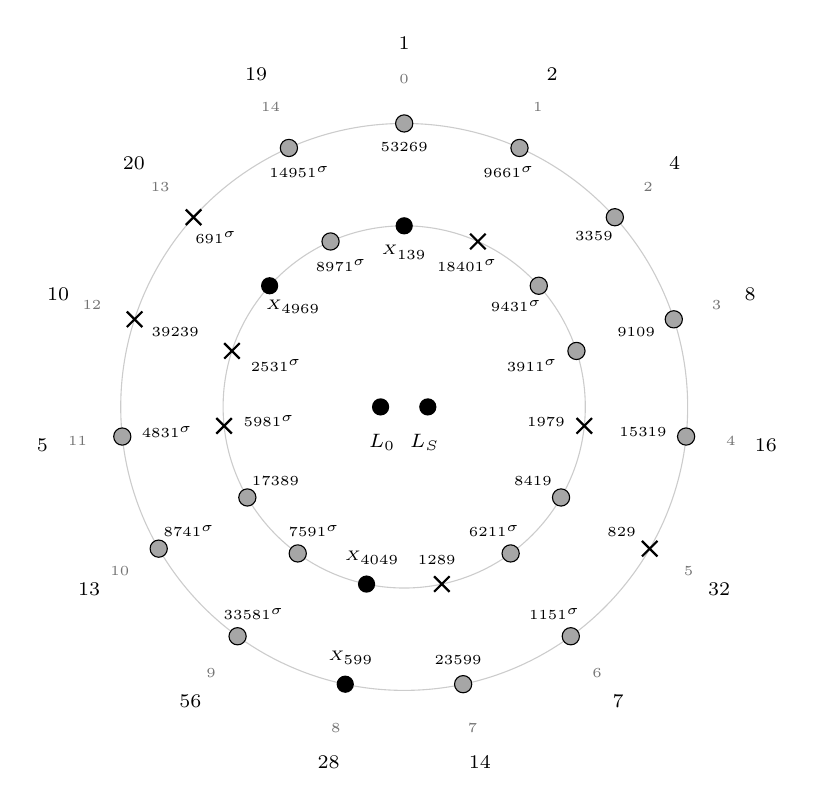
\begin{tikzpicture}[
  ext/.style={circle,fill=black,inner sep=2.2pt},
  rej/.style={cross out,draw=black,thick,inner sep=2.4pt},
  par/.style={circle,draw=black,fill=black!35,inner sep=2.2pt},
  une/.style={circle,draw=black!55,inner sep=2.2pt},
  lab/.style={font=\tiny,inner sep=1.2pt}]
\def\ri{2.3}\def\ro{3.6}
\draw[black!20] (0,0) circle (\ri);
\draw[black!20] (0,0) circle (\ro);
\foreach \h/\k in {0/1,1/2,2/4,3/8,4/16,5/32,6/7,7/14,8/28,9/56,10/13,11/5,12/10,13/20,14/19} {
  \pgfmathsetmacro{\a}{90-24*\h}
  \node[font=\scriptsize] at (\a:4.62) {$\k$};
  \node[font=\tiny,black!55] at (\a:4.17) {$\h$};
}
% anneau interieur : support {3,331}
\foreach \h/\s/\l in {0/ext/X_{139},1/rej/18401^{\sigma},2/par/9431^{\sigma},3/par/3911^{\sigma},4/rej/1979,5/par/8419,6/par/6211^{\sigma},7/rej/1289,8/ext/X_{4049},9/par/7591^{\sigma},10/par/17389,11/rej/5981^{\sigma},12/rej/2531^{\sigma},13/ext/X_{4969},14/par/8971^{\sigma}} {
  \pgfmathsetmacro{\a}{90-24*\h}
  \node[\s] at (\a:\ri) {};
  \node[lab,anchor=\a] at (\a:\ri-0.2) {$\l$};
}
% anneau exterieur : support {331}
\foreach \h/\s/\l in {0/par/53269,1/par/9661^{\sigma},2/par/3359,3/par/9109,4/par/15319,5/rej/829,6/par/1151^{\sigma},7/par/23599,8/ext/X_{599},9/par/33581^{\sigma},10/par/8741^{\sigma},11/par/4831^{\sigma},12/rej/39239,13/rej/691^{\sigma},14/par/14951^{\sigma}} {
  \pgfmathsetmacro{\a}{90-24*\h}
  \node[\s] at (\a:\ro) {};
  \node[lab,anchor=\a] at (\a:\ro-0.2) {$\l$};
}
\node[ext] at (-0.3,0) {}; \node[ext] at (0.3,0) {};
\node[font=\scriptsize] at (0,-0.45) {$\Lz\ \ \LS$};
\end{tikzpicture}

\caption{The $\sigma_{24}$-layer. Inner ring: the $15$ orbits of support $\{3,331\}$ (normalizer of order $460$); outer ring: their $15$ twins, of support $\{331\}$ (normalizer of order $920$); centre: the twin pair $(\Lz,\LS)$. Outside: hour $h$ (small) and smallest exponent $k$. Black disc: extremal (computer-assisted; \cite{Sak26} for the centre); cross: a vector of norm $6$ (proved); grey disc: partial survivor of a filter (of~\cite{Gau26} or of \S\ref{subsec:census}); open circle: not examined. A label $p^\sigma$ denotes the orbit of $P\sigma_{24}(P)$, for a prime $P$ of degree~$1$ above $p$; $p$ alone, that of a prime of degree~$2$ above $p$. Hours: proved without GRH (Corollary~\ref{cor:dial}).}\label{fig:dial}
\end{figure}

\subsection{The census of the layer}\label{subsec:census}
For each of the $30$ non-central orbits, a representative of small norm was sought among two families: prime ideals of degree $2$ above $p\equiv24\pmod{115}$, and ideals $P\sigma_{24}(P)$ with $P$ of degree $1$ above $p\equiv1\pmod{115}$; in both cases $\Nm(I)=p^2$. The cost of a sweep grows like $\sqrt{\Nm(I)}=p$: the ratio of the values of $|\Uc|$ for $X_{4969}$ and $X_{139}$ is $35.96$, against $4969/139=35.75$. A search up to $p=300\,000$ ($574$ primes, $21$~s) reaches all $30$ orbits. Table~\ref{tab:census} gives the cheapest representative of each orbit, by hour. The search used GRH to label the ideals; Corollary~\ref{cor:dial} certifies all the hours without GRH. The verdicts never depended on GRH.

\begin{table}[ht]
\caption{The $30$ non-central orbits of the $\sigma_{24}$-layer, by hour: cheapest known representative ($p$ means $\Nm(I)=p^2$; (a) a prime of degree $2$, (b) an ideal $P\sigma_{24}(P)$) and status. ``ext.'': extremal, computer-assisted; ``rej.'': vector of norm $6$, proved; ``part.'': partial survivor of a filter. An asterisk marks the filters of the night of October 16 to 17 (Table~\ref{tab:filtres}).}\label{tab:census}
\centering\small\setlength{\tabcolsep}{5pt}
\begin{tabular}{rr ll ll}
\toprule
& & \multicolumn{2}{c}{support $\{3,331\}$ (inner ring)} & \multicolumn{2}{c}{support $\{331\}$ (outer ring)} \\
\cmidrule(lr){3-4}\cmidrule(lr){5-6}
$h$ & $k$ & representative & status & representative & status \\
\midrule
$0$ & $1$ & $139$ (a) & ext.\ ($X_{139}$) & $53\,269$ (a) & part.* \\
$1$ & $2$ & $18\,401$ (b) & rej.* & $9\,661$ (b) & part.* \\
$2$ & $4$ & $9\,431$ (b) & part.* & $3\,359$ (a) & part. \\
$3$ & $8$ & $3\,911$ (b) & part.* & $9\,109$ (a) & part.* \\
$4$ & $16$ & $1\,979$ (a) & rej. & $15\,319$ (a) & part.* \\
$5$ & $32$ & $8\,419$ (a) & part.* & $829$ (a) & rej. \\
$6$ & $7$ & $6\,211$ (b) & part.* & $1\,151$ (b) & part.* \\
$7$ & $14$ & $1\,289$ (a) & rej. & $23\,599$ (a) & part.* \\
$8$ & $28$ & $4\,049$ (a) & ext.\ ($X_{4049}$) & $599$ (a) & ext.\ ($X_{599}$) \\
$9$ & $56$ & $7\,591$ (b) & part.* & $33\,581$ (b) & part.* \\
$10$ & $13$ & $17\,389$ (a) & part.* & $8\,741$ (b) & part.* \\
$11$ & $5$ & $5\,981$ (b) & rej.* & $4\,831$ (b) & part.\ ($5\,659$ (a)); part.* \\
$12$ & $10$ & $2\,531$ (b) & rej.* & $39\,239$ (a) & rej.* \\
$13$ & $20$ & $4\,969$ (a) & ext.\ ($X_{4969}$) & $691$ (b) & rej.\ (prop.~\ref{prop:temoin}) \\
$14$ & $19$ & $8\,971$ (b) & part.* & $14\,951$ (b) & part.* \\
\bottomrule
\end{tabular}
\end{table}

A complementary search, for prime ideals of degree~$1$ whose class has zero $45\,013$-component (about one prime in $45\,013$; cost $\sqrt p$ only, since $\Nm(P)=p$), was carried out up to $p\approx1.13\cdot10^9$ ($648\,833$ primes $p\equiv1\pmod{115}$, four slices, about $69$ hours of computation in total); it tests the vanishing of the $45\,013$-component in $\Cl(K_{44})$, under GRH. It found $9$ primes of the layer, and improves only one orbit: hour $10$ of the inner ring, by a prime above $p=157\,146\,581$, of cost $\sqrt p\approx12\,536$ instead of $17\,389$. For this prime, the label $c=318$ and the hour are certified by Proposition~\ref{prop:dial} ($e=1$), but the vanishing of the $45\,013$-component remains under GRH.

\emph{Filters of the night.} On the night of October~16 to~17, the program \texttt{Rang88CertZ} was run as a filter on the representatives, in Table~\ref{tab:census}, of $\nfiltres$ of the $\navant$ undecided orbits (all but that of $P_{3359}$, a partial survivor of a filter of~\cite{Gau26} with this same representative), on the author's computer: both sides in parallel, $5$ threads each, stopped at the first hit and capped at $12$ minutes. Every hit was checked exactly by a PARI/GP script that uses only the coordinates $(u,y)$ of the hit: the basis generates the ideal (up to Galois conjugation for a prime of degree~$2$, which does not change the orbit), the Gram matrix recomputed from $\alpha$ is integral, even, unimodular and positive definite, and the vector has integer coordinates and norm $6$. A rejection is counted only if this check succeeds entirely (exit code, final sentinel, complete count of checks, no error). Table~\ref{tab:filtres} gives the outcome: $\nrejets$ orbits are rejected, which is proved without GRH, and $\nsurv$ are partial survivors, about which nothing is proved. Each surviving filter went through $\projmin$ to $\projmax$ million short projections, both sides together; in~\cite[\S6.3]{Gau26}, the rejections of the same family occurred after $0.30$ to $0.43$ million short projections of side~$1$. \CONS

\begin{table}[ht]
\caption{Filters of the night of October 16 to 17, in the order of increasing cost. Projections: millions of short projections gone through, both sides together. For a rejection, the energies of the hit (short and fiber; sum $12$), and the side on which it occurred.}\label{tab:filtres}
\centering\small\setlength{\tabcolsep}{4pt}
\begin{tabular}{rl l l r r l}
\toprule
$h$ & ring & ideal & verdict & projections & time (s) & energies of the hit \\
\midrule
\lignesfiltresen
\bottomrule
\end{tabular}
\end{table}

\subsection{A heuristic: symmetry protects extremality}\label{subsec:heur}
The heuristic of~\cite[(Q2)]{Gau26} (Siegel mean, Poisson law on the orbits of short vectors) gives a lattice whose normalizer of $\langle\zeta\rangle$ has order $230$ a probability of about $4.4\%$ of being extremal. If the vectors of norm $\le6$ are distributed as in a lattice without extra symmetry, a normalizer of order $230m$ divides the number of their orbits by $m$, and the probability becomes about $0.044^{1/m}$: $21\%$ for the inner ring ($m=2$) and $46\%$ for the outer ring ($m=4$). \HEUR

Before the filters of \S\ref{subsec:census}, the data were small but suggestive. In the inner ring, three of the five decided orbits are extremal; in the outer ring, one of three; among the generic orbits of size $88$, none of the fifteen decided ideals of degree $1$ is (the four rejections of~\cite{Gau26} and the eleven new rejections of the control group). With these probabilities, the $22$ orbits of the layer then undecided would contain about $10\times0.21+12\times0.46\approx7.6$ further extremal lattices. \HEUR

The filters of \S\ref{subsec:census} give a first test. If the heuristic were right, and if a filter of this strength caught every non-extremal lattice, about $79\%$ of the inner orbits and $54\%$ of the outer orbits filtered would have been rejected. In fact $\nrejint$ of the $\nfiltint$ inner orbits and $\nrejext$ of the $\nfiltext$ outer orbits were rejected, whereas the filters of~\cite{Gau26} and of \S\ref{sec:audit} had rejected $15$ of the $17$ generic ideals of degree~$1$ they examined. \CONS

Under these two hypotheses, and if the orbits behaved independently with these common probabilities, a deviation at least as large would have a probability of about $\probint\%$ for the inner ring and $\probext\%$ for the outer ring (binomial law). This number does not measure the probability that the hypotheses are false: it only says that such a deviation would be rare if they were right, and a fluctuation in a small sample is not excluded. Two explanations are possible, without excluding a fluctuation or dependences between orbits: extremal lattices may be more frequent in the layer than the heuristic predicts, or the short vectors of its non-extremal lattices may be harder for a filter to reach. Moreover, if the number of short projections grows like $p$, as the comparison of $X_{139}$ and $X_{4969}$ suggests, a filter of fixed duration, which goes through $\projmin$ to $\projmax$ million of them (Table~\ref{tab:filtres}), covers a fraction of the enumeration that decreases like $1/p$: the survival of the most expensive orbits says less. Only complete sweeps can decide. \HEUR

With the representatives of Table~\ref{tab:census}, a cost of $0.0035\,p$ hours of a rented $32$-core machine for a complete execution of both sides (calibrated on $X_{4969}$), a quick rejection for a non-extremal lattice and two executions for an extremal one, the expected cost of this census was about $\coutavant$ hours before the filters of \S\ref{subsec:census}. For the $\nouvertes$ orbits still open, it is about $\coutheur$ hours with the same probabilities, and about $\couttous$ hours if they are all extremal. Beyond the layer, the $1\,023$ orbits fixed by $\sigma_{91}$ (support $\{45\,013\}$, normalizer of order $460$) would contain about two hundred, and the $507\,408$ generic orbits, at $4.4\%$, more than twenty thousand. These numbers are not results: the model was compared with only two cases in rank $56$, and it underestimated one of them. They say where to look. \HEUR

\section{Outlook}\label{sec:outlook}
\begin{enumerate}[label=\textup{(\arabic*)}]
\item \emph{The census of the layer.} Of the $\navant$ orbits undecided before the filters of \S\ref{subsec:census}, $\nrejets$ are now rejected. The other $\nouvertes$ can be settled by the same pipeline: each needs a complete sweep, stopped at the first hit for a non-extremal lattice, and two executions for an extremal one; the cheapest, that of $P_{1151}\sigma_{24}(P_{1151})$, would take about four hours of a rented $32$-core machine per execution. By~\cite[Rem.~2.6]{Gau26}, each new extremal lattice of the layer has a normalizer of $\langle\zeta\rangle$ of order $460$ or $920$ in its automorphism group.
\item \emph{Twins.} Theorem~\ref{thm:twins} shows that extremality is not a twin invariant. Four twin pairs are now decided: two pairs of extremal lattices, $(\Lz,\LS)$ and $(X_{4049},X_{599})$; one pair of non-extremal lattices, at hour $12$ ($P_{2531}\sigma_{24}(P_{2531})$ and $P_{39239}$, rejected by the filters of \S\ref{subsec:census}); and the discordant pair of Theorem~\ref{thm:twins}. Whether extremality is \emph{correlated} between twins is open. The filters leave five pairs with one member rejected and the other a partial survivor: the inner member is rejected at hours $1$, $4$, $7$ and $11$, the outer one at hour $5$. The twin of $X_{139}$, $P_{53269}$, survived a filter that covered only a small fraction of its enumeration. Complete sweeps of these survivors would show whether discordant pairs are frequent.
\item \emph{The $\sigma_{91}$-layer.} Proposition~\ref{prop:cyclic} has an analogue for the classes fixed by $\sigma_{91}$: they form the cyclic group $\Cl_{45\,013}$, with $1\,023$ non-trivial orbits of size $44$. Its census requires cheap representatives, which a search of the kind of \S\ref{subsec:census} would provide.
\item \emph{Consolidation.} An independent implementation of the enumeration remains the main missing step (question (Q1) of~\cite{Gau26}); the recount of \S\ref{sec:audit} by \texttt{qfminim} is a first, non-certifying, step in that direction.
\end{enumerate}

\section*{Data, methods and declarations}
\emph{Data.} The input files, receipts, logs, verifiers and certificates of this addendum will be added to the public repository of~\cite{Gau26}, in the folders \texttt{addendum} (twin certificates, labels without GRH, filters of \S\ref{subsec:census}), \texttt{verification\_P4969}, \texttt{verification\_P4049}, \texttt{calcul\_externe\_resultats\_20261015} and \texttt{contre\_audit\_20261016}. The computations used PARI/GP 2.15.4, Python~3 in exact integer and rational arithmetic, and Java (OpenJDK 11, 17 and 21). The sweeps ran on rented Scaleway instances POP2-HC-32C-64G.

\emph{Use of artificial intelligence.} As for~\cite{Gau26}, the author was helped by two assistants, Claude Opus~5.5 (Anthropic) and Astra (OpenAI), who are not authors. The text, the programs and the certificates were written, and the computations conducted, with Claude Opus~5.5. Astra designed part of the audit plan, had the records listed in \S\ref{subsec:review} attacked and reread, and found the defects reported there. On October~17, Astra also read, without executing them, the argument of Proposition~\ref{prop:dial} with its two verifiers, and the launcher, the witness verifier and the audit of the filters of \S\ref{subsec:census}. It confirmed the argument. It required the hypothesis that $\q$ be prime to the auxiliary primes, and it found gaps in the contract of the first Python verifier (no primality test, no check of $e$ against the type, no fixed list of targets, floating-point square roots), a defect in the first launcher, which recorded a hit as a rejection whatever the outcome of the exact check, and a contract of the witness verifier that was too broad, now restricted to the two forms of ideals actually used. All were corrected, and every rejection was re-verified. Astra also read the twin and same-orbit certificates and the witness of norm $6$ of $P_{691}\sigma_{24}(P_{691})$, without executing them: it found no mathematical defect in the positive chain of Theorem~\ref{thm:twins}, and asked for the four elements $\delta$ of the same-orbit certificates to be exported, which was done. The census and the other results of \S\ref{sec:layer} have not been reviewed by Astra.

The author takes scientific responsibility for the entire content. This addendum has not been reviewed by a human specialist.

\begin{thebibliography}{NS}
\bibitem[Gau26]{Gau26}
I.~Gauvin, \emph{Even unimodular ideal lattices of rank $88$ over $\Q(\zeta_{115})$}, preprint, October 15, 2026 (arXiv identifier pending); French original: \emph{R\'eseaux id\'eaux pairs unimodulaires de rang $88$ sur $\Q(\zeta_{115})$}. Repository: \url{https://github.com/Katabolanga/rang88-reseaux-ideaux}.

\bibitem[NS]{NS}
G.~Nebe, N.~J.~A.~Sloane, \emph{A Catalogue of Lattices}, \url{https://www.math.rwth-aachen.de/~Gabriele.Nebe/LATTICES/}.

\bibitem[Sak26]{Sak26}
R.~Sakamoto, \emph{Two extremal even unimodular lattices of rank $88$}, preprint arXiv 2609.15633, version~2 of September 27, 2026.
\end{thebibliography}

\end{document}
